\section{Problema: Riconoscimento dei Segnali Stradali}
In questa era dell'Intelligenza Artificiale, gli esseri umani stanno diventando sempre più dipendenti dalla tecnologia. Con la tecnologia avanzata, aziende multinazionali come Google, Tesla e molte altre stanno lavorando per automatizzare i veicoli, cercando di creare veicoli autonomi o senza conducente il più possibile precisi. Infatti le auto a guida autonoma, in cui il veicolo stesso si comporta come un'autista, non ha bisogno di alcuna guida umana per circolare sulla strada. Non è sbagliato preoccuparsi degli aspetti legati alla sicurezza, in quanto è sempre presente la possibilità di incidenti. Ma sappiamo che nessuna macchina è più precisa degli esseri umani. I ricercatori stanno eseguendo numerosi algoritmi per garantire una sicurezza stradale al 100$\%$. Fra questi, un algoritmo fondamentale è il \textbf{Riconoscimento dei Segnali Stradali}.

Quando si è in strada, si vedono vari segnali stradali come curve a sinistra o a destra, limiti di velocità, divieto di sorpasso ai veicoli pesanti, divieto di accesso, attraversamento pedonale per bambini, ecc., che è necessario seguire per una guida sicura. Allo stesso modo, i veicoli autonomi devono anche interpretare questi segnali e prendere decisioni per garantire la precisione. Per riconoscere a quale categoria appartiene un segnale stradale è necessario quindi classificarli.

In questo progetto di Machine Learning, costruiremo un modello per la classificazione dei segnali stradali presenti nell'immagine in molte categorie utilizzando una rete neurale convoluzionale (CNN).

In figura \ref{Esempio} è presente un esempio visivo che descrive il problema. 
\vspace{+1truecm}
\begin{figure}[H]
    \centering
    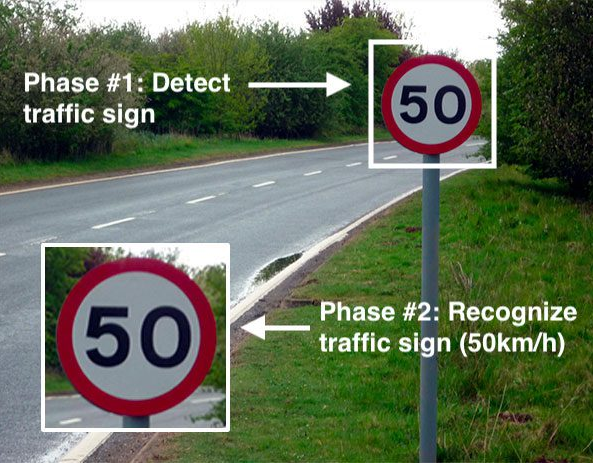
\includegraphics[scale=0.6]{Build/Immagine.png}
    \caption{Esempio}
    \label{Esempio}
\end{figure}

\newpage

\subsection{Dataset}

Il dataset completo delle immagini, scaricabile al link \url{https://www.kaggle.com/datasets/meowmeowmeowmeowmeow/gtsrb-german-traffic-sign}, è composto da più di 50.000 foto di vari segnali stradali (limiti di velocità, attraversamenti, segnali stradali, ecc.), con una dimensione totale di circa 560 MB. \\ Per questo lavoro nello specifico sono state utilizzate le immagini contenute nel percorso\\ $\text{DITS}$, con una dimesione di 450 MB.

\begin{figure}[H]
    \centering
    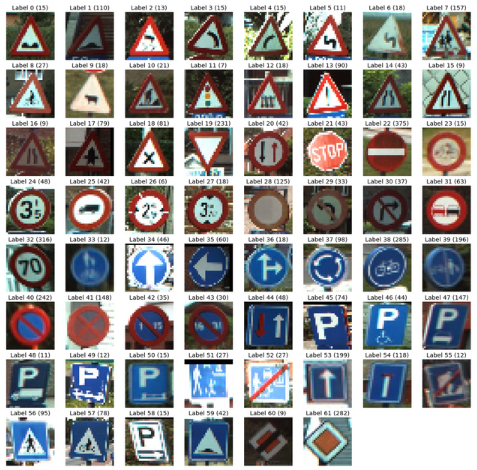
\includegraphics[scale=0.7]{Build/Immagine2.png} 
    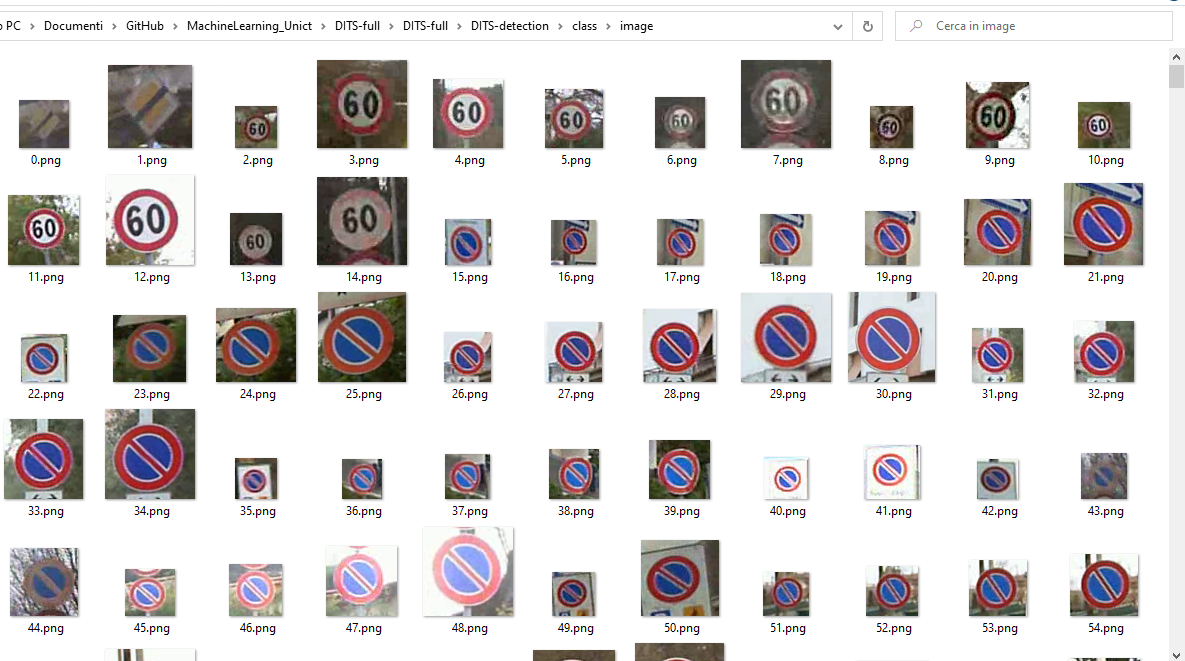
\includegraphics[scale=0.4]{Build/Dataset.png}
    \caption{Esempi visuali dei dati}
    \label{fig:enter-label}
\end{figure}

Del dataset sono presenti due versioni una in cui i segnali sono divisi per segnale specifico e un'ultima da me scelta la divisione per macro categoria di segnale, in questo modo i segnali del dataset si dividono nelle loro 3 macrocategorie, a cui è poi stata aggiunta attraverso uno script una quarta categoria, arrivando ad avere le seguenti categorie:

\begin{itemize}
    \item Divieto
    \item Pericolo
    \item Obbligo    
    \item Backgroud (utile per un secondo scopo)
\end{itemize}